\documentclass{classrep}
\usepackage[utf8]{inputenc}
\frenchspacing

\usepackage{graphicx}
\usepackage[usenames,dvipsnames]{color}
\usepackage[hidelinks]{hyperref}
\usepackage[section]{placeins}
\usepackage{float}
\usepackage{amsmath, amssymb, mathtools}

\setlength{\abovecaptionskip}{0pt}
\setlength{\belowcaptionskip}{0pt}

\usepackage{fancyhdr, lastpage}
\pagestyle{fancyplain}
\fancyhf{}
\renewcommand{\headrulewidth}{0pt}
\cfoot{\thepage\ / \pageref*{LastPage}}


\studycycle{Informatyka, studia dzienne, I st.}
\coursesemester{IV}

\coursename{Inteligentna Analiza Danych}
\courseyear{2017/2018}

\courseteacher{mgr inż. Paweł Tarasiuk}
\coursegroup{piątek, 10:15}

\author{%
\studentinfo[210320@edu.p.lodz.pl]{Michał Sobczyk}{210320}\\
  \studentinfo[215145@edu.p.lodz.pl]{Michał Chudzik}{215145}
  %
}

\title{Zadanie 1}

\begin{document}
\maketitle
\thispagestyle{fancyplain}

\section{Cel}
	Celem zadania jest implementacja i zbadania sieci neuronowej. Implementacja składa się ze skalowalnej sieci neuronowej wykorzystującej wsteczną propagację błędów jako metodę nauki oraz momentum.

\section{Wprowadzenie}
	\textbf{Perceptron wielowarstwowy}-  głównym elementem są neurony przetwarzające. Każdy neuron posiada dowolną liczbę wejść oraz jedno wyjście. Neurony są pogrupowane w warstwy, gdzie każde dwie sąsiednie warstwy są połączone iloczynem kartezjańskim. Na wejście neuronu trafiają wyjścia wszystkich neuronów z warstwy poprzedniej.


Przetwarzanie wymaga obliczonych wcześniej wartości wyjściowych z poprzednich warstw. Ten proces dany jest poniższym wzorem
\begin{equation} \label{eq:feedforward}
	a_{t+1} = \sigma ( Wa_t + b),
\end{equation}
gdzie $a_{t+1}$ jest macierzą wyjścia warstwy neuronowej, $a_t$ macierzą wejścia warstwy neuronowej, W macierzą wag, b macierzą biasów a $\sigma$ jest funkcją aktywacji daną wzorem
\begin{equation} \label{eq:activation}
	\sigma = \frac{1}{1 + e^{-x}}.
\end{equation}


Proces nauki jest wykonany za pomocą metody najmniejszych spadków. Aktualizacja wag dana jest wzorem
\begin{equation} \label{eq:generalBackPropagationWeight}
	w_i = w_i - \lambda \cdot \frac{\delta E}{\delta w_i},
\end{equation}
gdzie $w_i$ jest wagą która jest aktualizowana, $\lambda$ współczynnik uczenia, $E_{total}$ dany jest wzorem
\begin{equation} \label{eq:totalError}
	E = \sum \frac{1}{2}(target - output)^2,
\end{equation}
gdzie output oznacza wynik końcowy sieci neuronowej a target oczekiwaną wartość tegoż wyniku.


Aktualizacja biasów zachodzi w sposób
\begin{equation} \label{eq:generalBackPropagationBias}
	b_i = b_i - \lambda \cdot \frac{\delta E}{\delta b_i},
\end{equation}
gdzie $b_i$ jest zmienianym biasem.

\section{Opis implementacji}
Aplikacja została stworzona w języku Python3 przy użyciu dodatkowych modułów bibliotecznych takich jak:
		\begin{itemize}
			\item matplotlib - generowanie wykresów
			\item sklearn - import wybranych zbiorów danych oraz algorytm KNN
			\item urllib - pobranie wybranego zbioru danych nie zawartego w bibliotece sklearn
		\end{itemize}

\section{Materiały i metody}
Analiza danych została przeprowadzona na zbiorze opisującym wina irysy \cite{irisdataset} oraz nasiona \cite{seedsdataset}


Eksperymenty 1 - 3 zostały przeprowadzone za pomocą sieci neuronowej dla zbioru Iris. Zasób treningowy liczył 100 losowych krotek, a reszta (40) została użyta do przetestowania klasyfikacji. Dla omawianych eksperymentów algorytm wykonywał 1000 iteracji.\\


\textbf{Eksperyment 1 - Zbiór irysów}\\
		Wpływ ilości neuronów na uczenie.\\
		learning rate = 0.5\\
		momentum = 0.0\\
		size - rozłożenie neuronów
		\begin{itemize}
			\item \textbf{E1.1}
			 size = [4, 2, 3]
			\item \textbf{E1.2} 
			size = [4, 7, 3]
			\item \textbf{E1.3}
			size = [4, 12, 3]
			\item \textbf{E1.4}
			size = [4, 20, 3]\\
		\end{itemize}
	
	\textbf{Eksperyment 2 - Zbiór irisów}\\
		Wpływ learning rate na uczenie.\\
		size = [4, 2, 3]\\
		momentum =  0.0
		\begin{itemize}
			\item \textbf{E2.1}
			 learning rate = 0.2
			\item \textbf{E2.2} 
			learning rate = 0.4
			\item \textbf{E2.3}
			learning rate = 0.6
			\item \textbf{E2.4}
			learning rate = 0.8\\
		\end{itemize}
	
	\textbf{Eksperyment 3 - Zbiór irysów}\\
		Wpływ wartości momentum na uczenie.\\
		size = [4, 2, 3]\\
		learning rate = 0.2
		\begin{itemize}
			\item \textbf{E3.1}
			 momentum = 0.3
			\item \textbf{E3.2} 
			momentum = 0.5
			\item \textbf{E3.3}
			momentum = 0.7
			\item \textbf{E3.4}
			momentum = 0.9\\
		\end{itemize}

Eksperymenty 4 - 6 zostały przeprowadzone za pomocą sieci neuronowej dla zbioru Seeds. Zasób treningowy liczył 140 losowych krotek, a reszta 69 została użyta do przetestowania klasyfikacji. \\


	\textbf{Eksperyment 4 - Zbiór Seeds.}\\
		Wpływ liczby iteracji na uczenie.\\
		size = [7, 7, 3]\\
		learning rate = 0.5\\
		momentum = 0.3
		\begin{itemize}
			\item \textbf{E4.1}
			 iterations = 500
			\item \textbf{E4.2} 
			iterations = 1500
			\item \textbf{E4.3}
			iterations = 5000\\
		\end{itemize}

\textbf{Eksperyment 5 - Zbiór Seeds.}\\
		Wpływ wartości learning rate na uczenie.\\
		size = [7, 7, 3]\\
		iterations = 2000\\
		momentum = 0.0
		\begin{itemize}
			\item \textbf{E5.1}
			 learning rate = 0.3
			\item \textbf{E5.2} 
			learning rate = 0.5
			\item \textbf{E5.3}
			learning rate = 0.8\\
		\end{itemize}

\textbf{Eksperyment 6 - Zbiór Seeds.}\\
		Wpływ wartości momentum na uczenie.\\
		size = [7, 7, 3]\\
		iterations = 2000\\
		learning rate = 0.3
		\begin{itemize}
			\item \textbf{E6.1}
			 momentum = 0.1
			\item \textbf{E6.2} 
			momentum = 0.5
			\item \textbf{E6.3}
			momentum = 0.9\\
		\end{itemize}

Eksperymenty 7 - 10 zostały przeprowadzone dla klasyfikatora KNearestNeighbours. Połowa zbioru jest danymi testowymi, druga połowa danymi testowanymi.

\textbf{Eksperyment 7 - Zbiór irysów}\\
		Wpływ ilosci sąsiadów na jakosć uczenia się.
		\begin{itemize}
			\item \textbf{E7.1}
			 k = 5
			\item \textbf{E7.2} 
			k = 10
			\item \textbf{E7.3}
			k = 15
			\item \textbf{E7.4}
			k = 20\\
		\end{itemize}

	\textbf{Eksperyment 8 - Zbiór irysów}\\
		Dokładnosć uczenia się na kllasyfikacji zbioru danych testowych - używanych przez algoytm do nauki. Zmienna liczba k.
		\begin{itemize}
			\item \textbf{E8.1}
			 k = 5
			\item \textbf{E8.2} 
			k = 10
			\item \textbf{E8.3}
			k = 20
			\item \textbf{E8.4}
			k = 1
		\end{itemize}

	\textbf{Eksperyment 9 - Zbiór nasion}\\	
		Dokładnosć uczenia się na kllasyfikacji zbioru danych testowych - używanych przez algoytm do nauki. Zmienna liczba k.
		\begin{itemize}
			\item \textbf{E9.1}
			 k = 1
			\item \textbf{E9.2} 
			k = 5
			\item \textbf{E9.3}
			k = 10
			\item \textbf{E9.4}
			k = 20
		\end{itemize}
	\textbf{Eksperyment 10 - Zbiór nasion}\\	
		Dokładnosć uczenia się dla różnych wag. Rozpatrywane są: równoważne, dystansowe.
		\begin{itemize}
			\item \textbf{E9.1}
			k = 1
			\item \textbf{E9.2} 
			k = 20
			\item \textbf{E9.3} 
			k = 100
		\end{itemize}

\section{Wyniki}

\subsection{Eksperyment 1}
		\begin{figure}[H]
			\begin{minipage}{0.5\linewidth}
				\centering
				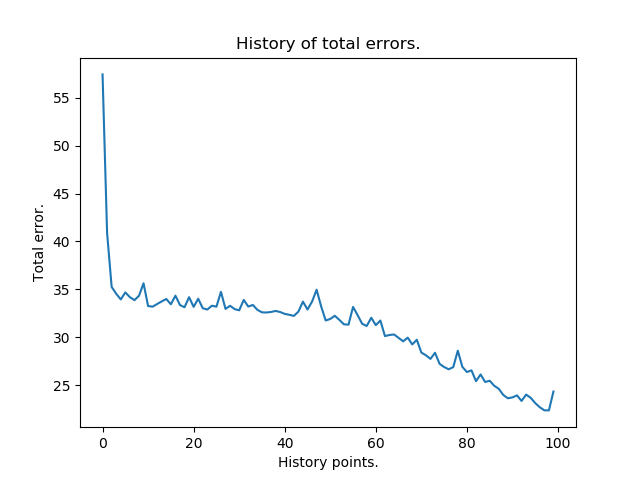
\includegraphics[scale=0.25]{iris_nn_s2.png}
				\caption{E1.1 Test rate  0.78}
			\end{minipage}
			\begin{minipage}{0.5\linewidth}
				\centering
				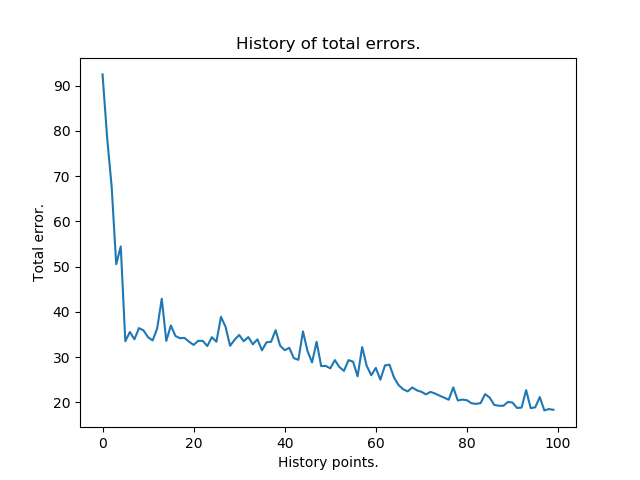
\includegraphics[scale=0.25]{iris_nn_s7.png}
				\caption{E1.2 Test rate  0.82}
				\label{E1.2}
			\end{minipage}
			\begin{minipage}{0.5\linewidth}
				\centering
				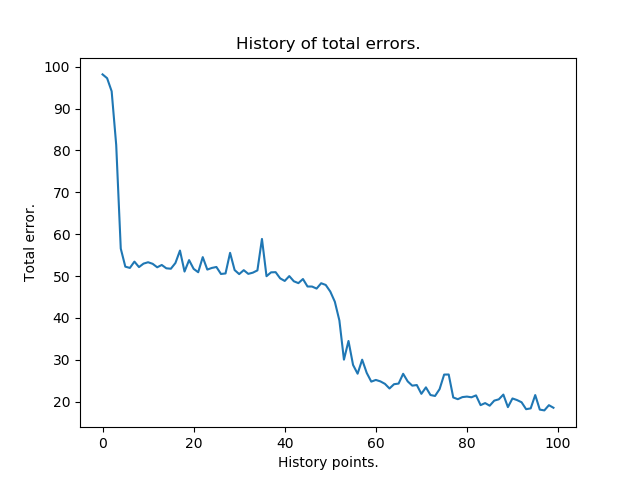
\includegraphics[scale=0.25]{iris_nn_s12.png}
				\caption{E1.3 Test rate  0.78}
			\end{minipage}
			\begin{minipage}{0.5\linewidth}
				\centering
				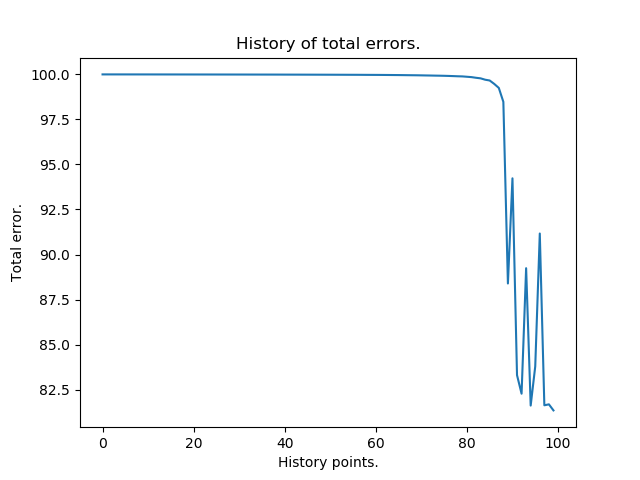
\includegraphics[scale=0.25]{iris_nn_s20.png}
				\caption{E1.4 Test rate  0.42}
			\end{minipage}
		\end{figure}
		\FloatBarrier
	\subsection{Eksperyment 2}
		\begin{figure}[H]
			\begin{minipage}{0.5\linewidth}
				\centering
				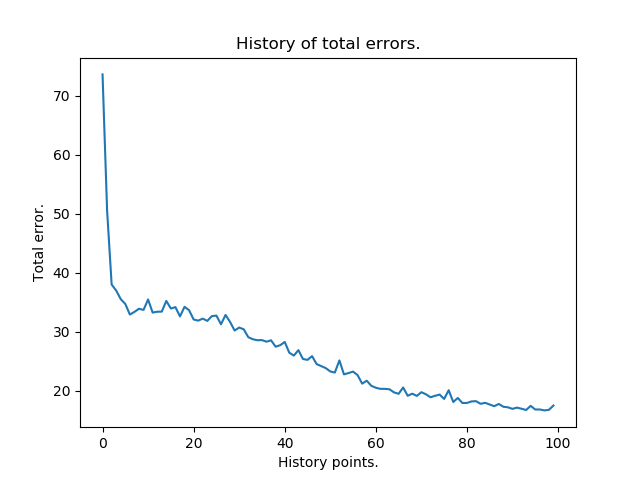
\includegraphics[scale=0.25]{iris_nn_l2.png}
				\caption{E2.1 Test rate  0.3}
			\end{minipage}
			\begin{minipage}{0.5\linewidth}
				\centering
				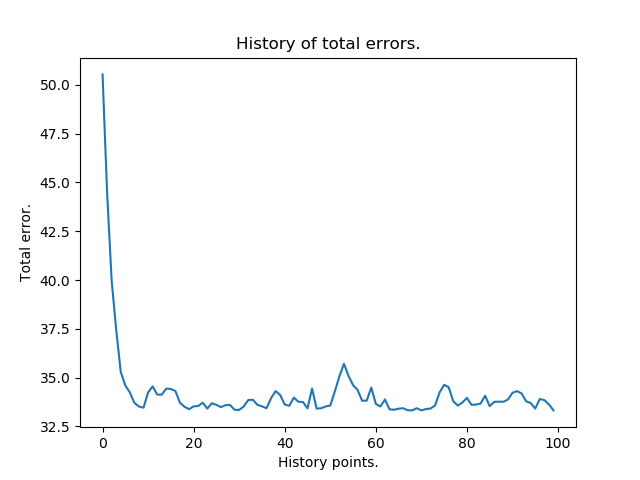
\includegraphics[scale=0.25]{iris_nn_l4.png}
				\caption{E2.2 Test rate  0.7}
				\label{E2.2}
			\end{minipage}
			\begin{minipage}{0.5\linewidth}
				\centering
				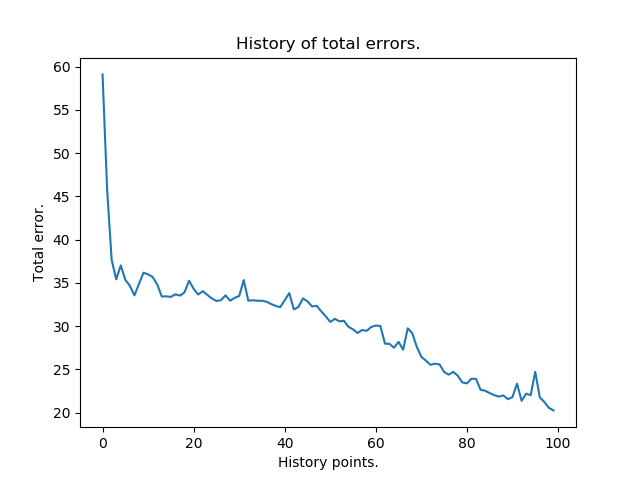
\includegraphics[scale=0.25]{iris_nn_l6.png}
				\caption{E2.3 Test rate  0.7}
			\end{minipage}
			\begin{minipage}{0.5\linewidth}
				\centering
				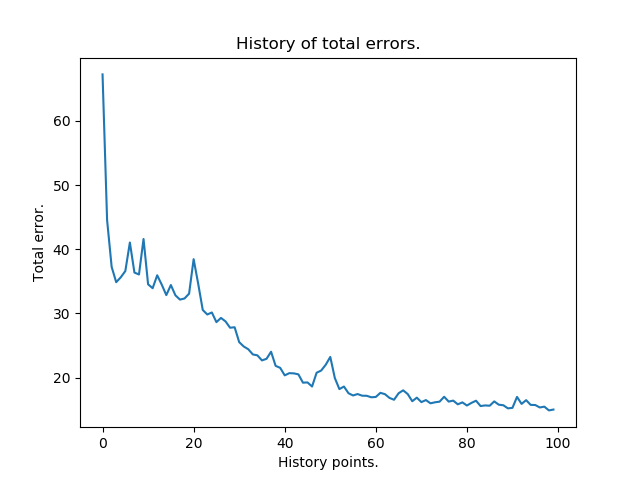
\includegraphics[scale=0.25]{iris_nn_l8.png}
				\caption{E2.4 Test rate  0.64}
			\end{minipage}
		\end{figure}
		\FloatBarrier
	\subsection{Eksperyment 3}
		\begin{figure}[H]
			\begin{minipage}{0.5\linewidth}
				\centering
				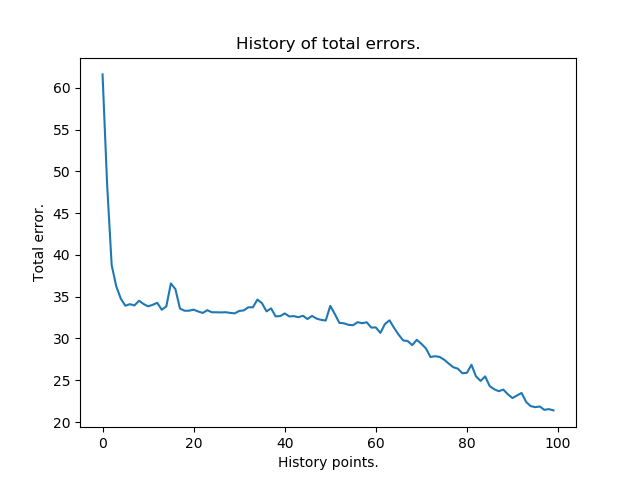
\includegraphics[scale=0.25]{iris_nn_m3.png}
				\caption{E3.1 Test rate  0.64}
			\end{minipage}
			\begin{minipage}{0.5\linewidth}
				\centering
				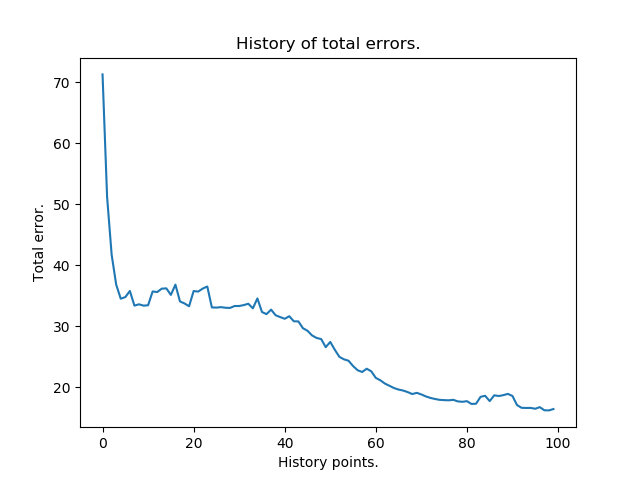
\includegraphics[scale=0.25]{iris_nn_m5.png}
				\caption{E3.2 Test rate  0.92}
				\label{E3.2}
			\end{minipage}
			\begin{minipage}{0.5\linewidth}
				\centering
				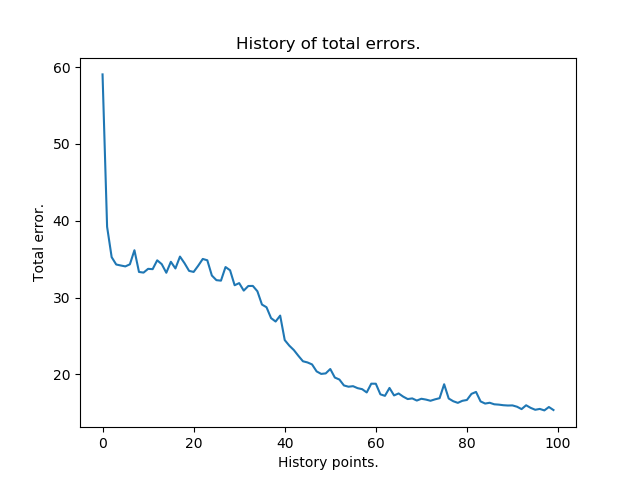
\includegraphics[scale=0.25]{iris_nn_m7.png}
				\caption{E3.3 Test rate  0.9}
				\label{E3.3}
			\end{minipage}
			\begin{minipage}{0.5\linewidth}
				\centering
				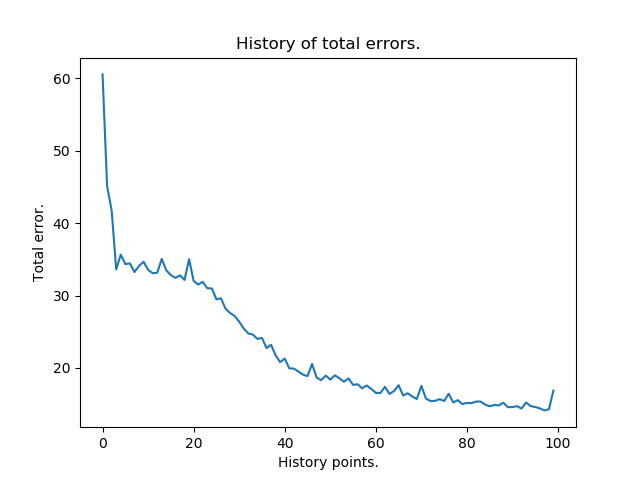
\includegraphics[scale=0.25]{iris_nn_m9.png}
				\caption{E3.4 Test rate  0.74}
				\label{E3.4}
			\end{minipage}
		\end{figure}
		\FloatBarrier
	\subsection{Eksperyment 4}
		\begin{figure}[H]
			\begin{minipage}{0.5\linewidth}
				\centering
				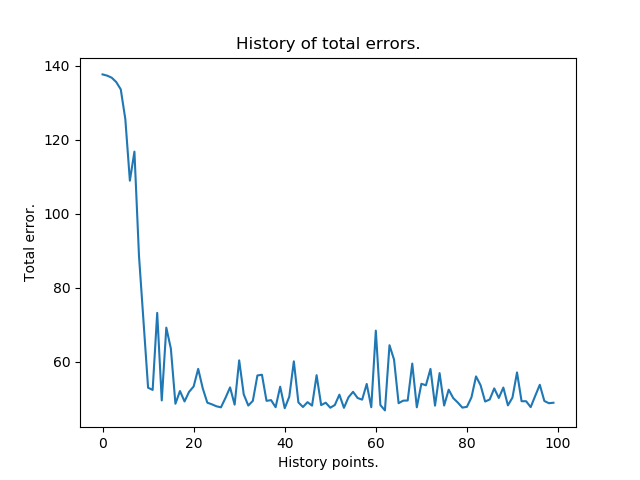
\includegraphics[scale=0.25]{seeds_nn_i500.png}
				\caption{E4.1 Test rate  0.34}
			\end{minipage}
			\begin{minipage}{0.5\linewidth}
				\centering
				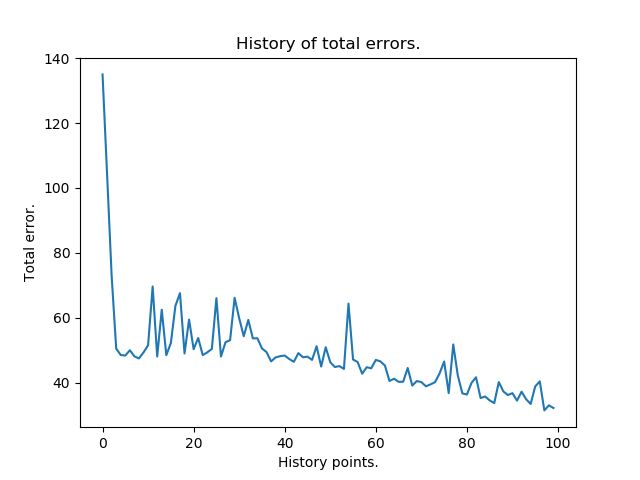
\includegraphics[scale=0.25]{seeds_nn_i1500.png}
				\caption{E4.2 Test rate  0.63}
				\label{E4.2}
			\end{minipage}
			\begin{minipage}{0.5\linewidth}
				\centering
				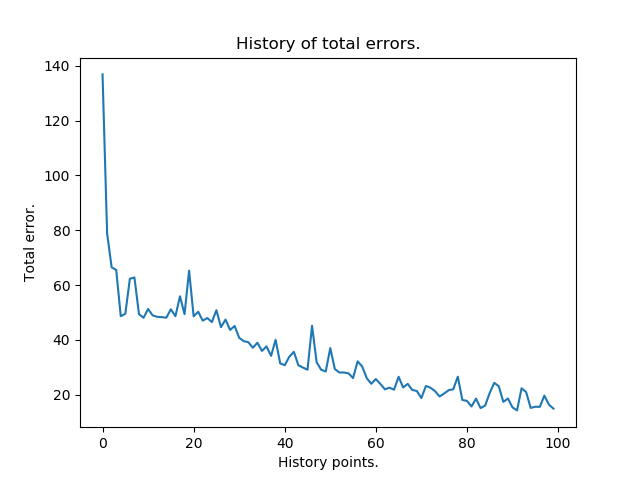
\includegraphics[scale=0.25]{seeds_nn_i5000.png}
				\caption{E4.3 Test rate  0.87}
				\label{E4.3}
			\end{minipage}
		\end{figure}
		\FloatBarrier
	\subsection{Eksperyment 5}
		\begin{figure}[H]
			\begin{minipage}{0.5\linewidth}
				\centering
				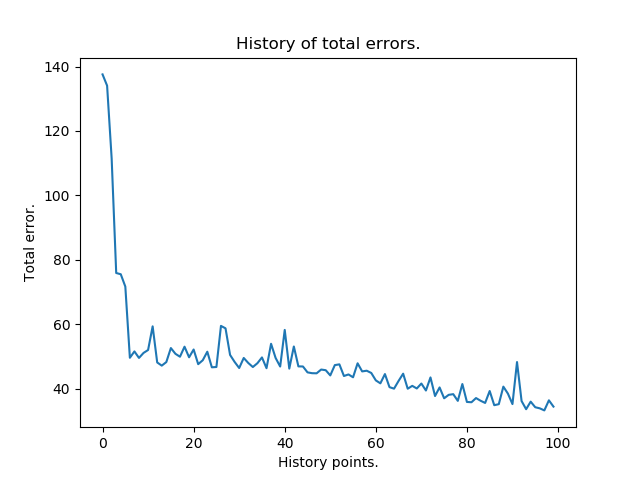
\includegraphics[scale=0.25]{seeds_nn_l2.png}
				\caption{E5.1 Test rate  0.30}
			\end{minipage}
			\begin{minipage}{0.5\linewidth}
				\centering
				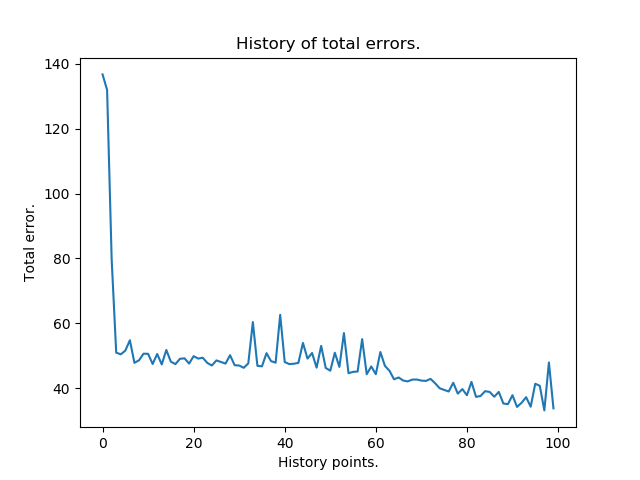
\includegraphics[scale=0.25]{seeds_nn_l5.png}
				\caption{E5.2 Test rate  0.60}
				\label{E5.2}
			\end{minipage}
			\begin{minipage}{0.5\linewidth}
				\centering
				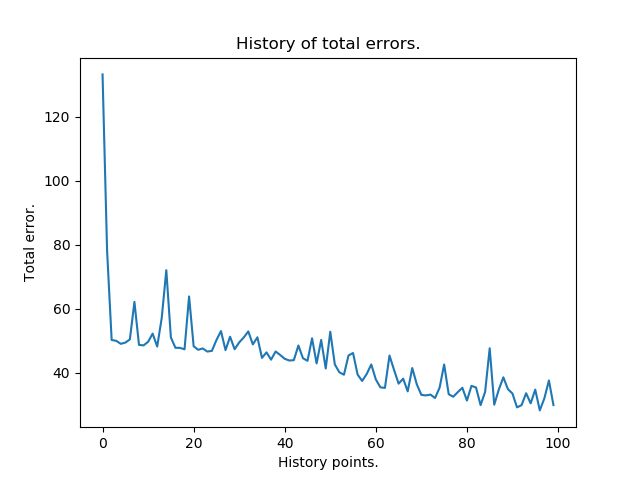
\includegraphics[scale=0.25]{seeds_nn_l8.png}
				\caption{E5.3 Test rate  0.68}
				\label{E5.3}
			\end{minipage}
		\end{figure}
		\FloatBarrier
	\subsection{Eksperyment 6}
		\begin{figure}[H]
			\begin{minipage}{0.5\linewidth}
				\centering
				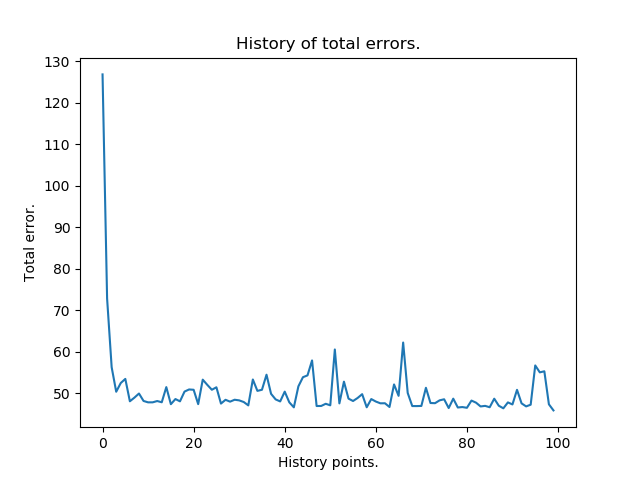
\includegraphics[scale=0.25]{seeds_nn_m1.png}
				\caption{E6.1 Test rate  0.39}
			\end{minipage}
			\begin{minipage}{0.5\linewidth}
				\centering
				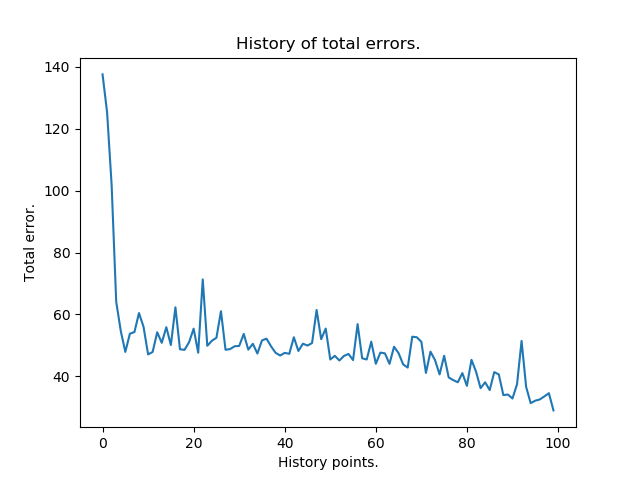
\includegraphics[scale=0.25]{seeds_nn_m5.png}
				\caption{E6.2 Test rate  0.68}
				\label{E6.2}
			\end{minipage}
			\begin{minipage}{0.5\linewidth}
				\centering
				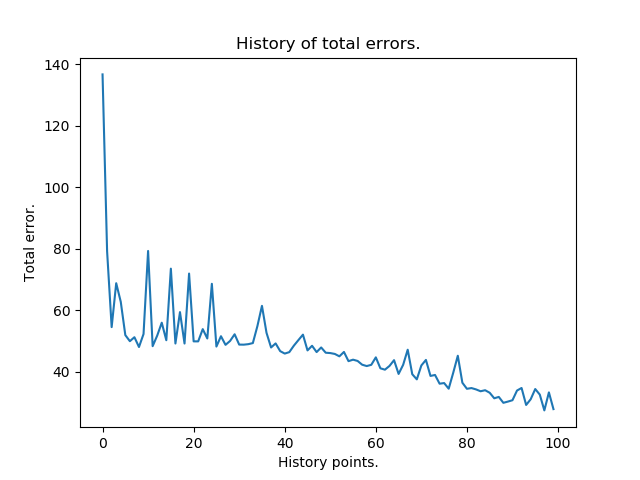
\includegraphics[scale=0.25]{seeds_nn_m9.png}
				\caption{E6.3 Test rate  0.78}
				\label{E6.3}
			\end{minipage}
		\end{figure}
		\FloatBarrier
	\subsection{Eksperyment 7}
		\begin{figure}[H]
			\begin{minipage}{0.5\linewidth}
				\centering
				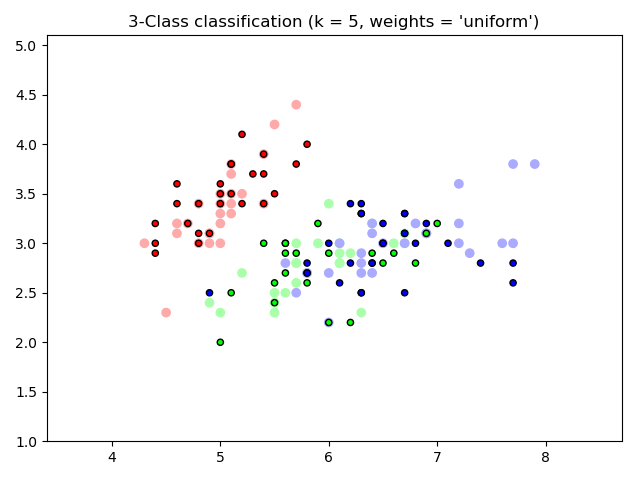
\includegraphics[scale=0.25]{KNN_iris_7_1.png}
				\caption{E7.1 accuracy = 98.65 \%}
			\end{minipage}
			\begin{minipage}{0.5\linewidth}
				\centering
				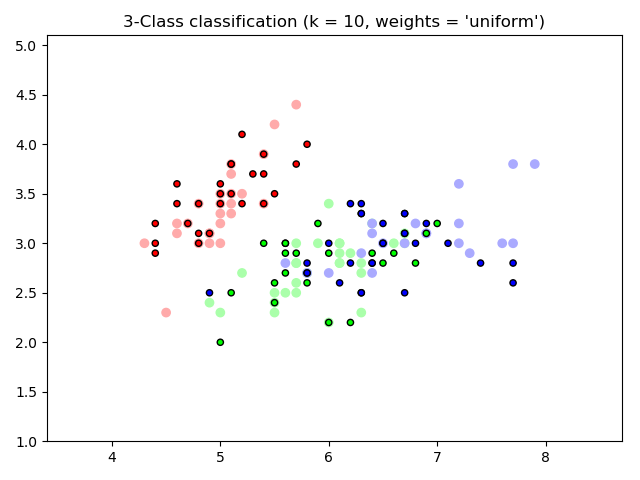
\includegraphics[scale=0.25]{KNN_iris_7_2.png}
				\caption{E7.2 accuracy = 91.89 \%}
				\label{E7.2}
			\end{minipage}
			\begin{minipage}{0.5\linewidth}
				\centering
				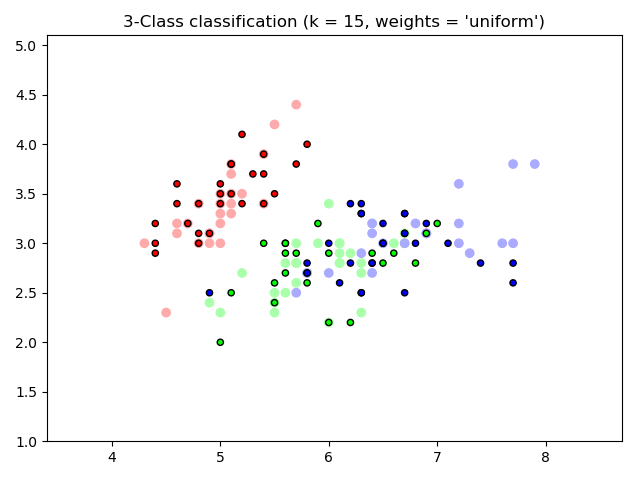
\includegraphics[scale=0.25]{KNN_iris_7_3.png}
				\caption{E7.3 accuracy = 91.89 \%}
				\label{E7.3}
			\end{minipage}
			\begin{minipage}{0.5\linewidth}
				\centering
				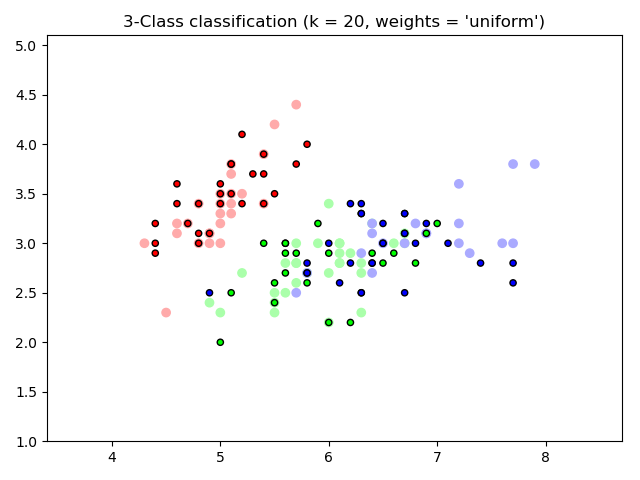
\includegraphics[scale=0.25]{KNN_iris_7_4.png}
				\caption{E7.4 accuracy = 93.24 \%}
				\label{E7.4}
			\end{minipage}
		\end{figure}
		\FloatBarrier
	\subsection{Eksperyment 8}
		\begin{figure}[H]
			\begin{minipage}{0.5\linewidth}
				\centering
				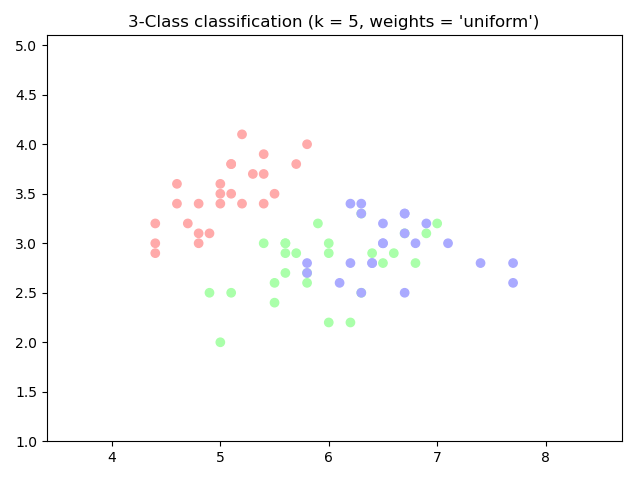
\includegraphics[scale=0.25]{KNN_iris_8_1.png}
				\caption{E8.1 accuracy = 97,33 \%}
			\end{minipage}
			\begin{minipage}{0.5\linewidth}
				\centering
				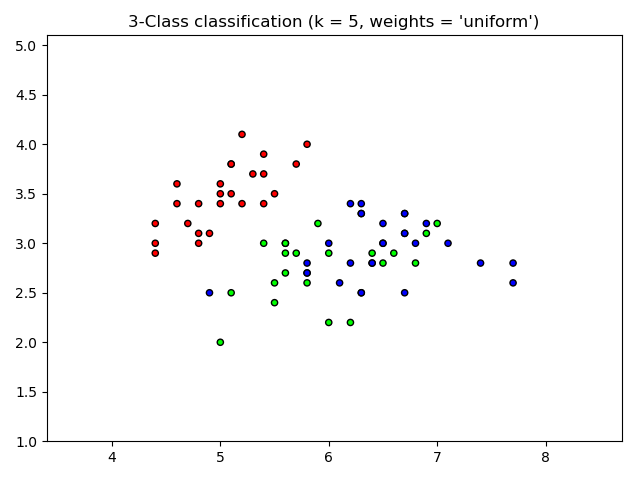
\includegraphics[scale=0.25]{KNN_iris_8_2.png}
				\caption{E8.1 accuracy = 97,33 \%}
				\label{E8.1}
			\end{minipage}
			\begin{minipage}{0.5\linewidth}
				\centering
				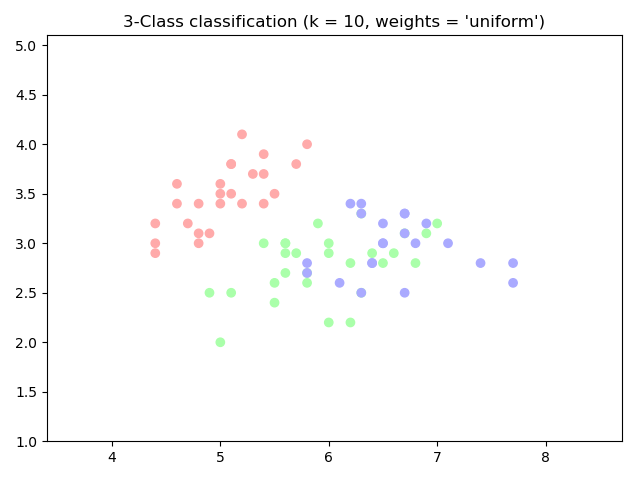
\includegraphics[scale=0.25]{KNN_iris_8_3.png}
				\caption{E8.2 accuracy = 96.00 \%}
				\label{E8.2}
			\end{minipage}
			\begin{minipage}{0.5\linewidth}
				\centering
				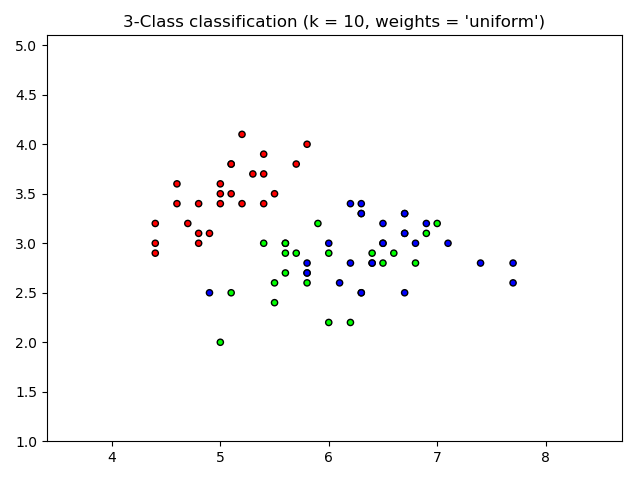
\includegraphics[scale=0.25]{KNN_iris_8_4.png}
				\caption{E8.2 accuracy = 96.00 \%}
				\label{E8.2}
			\end{minipage}
			\begin{minipage}{0.5\linewidth}
				\centering
				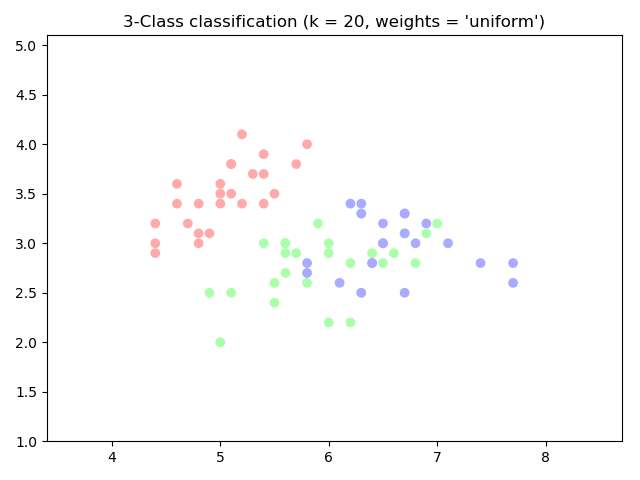
\includegraphics[scale=0.25]{KNN_iris_8_5.png}
				\caption{E8.3 accuracy = 96.00 \%}
				\label{E8.3}
			\end{minipage}
			\begin{minipage}{0.5\linewidth}
				\centering
				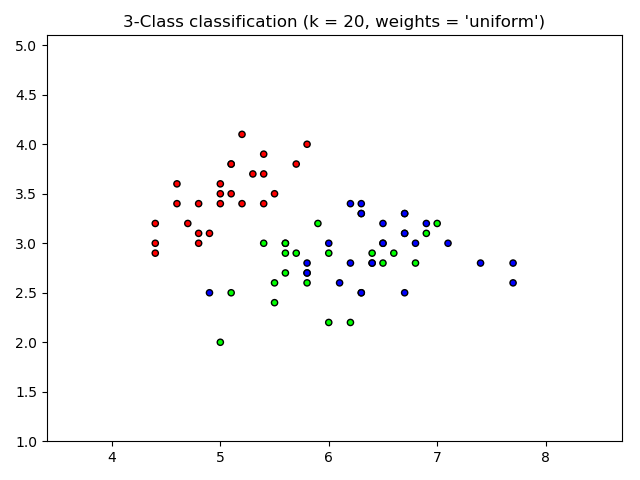
\includegraphics[scale=0.25]{KNN_iris_8_6.png}
				\caption{E8.3 accuracy = 96.00 \%}
				\label{E8.3}
			\end{minipage}
			\begin{minipage}{0.5\linewidth}
				\centering
				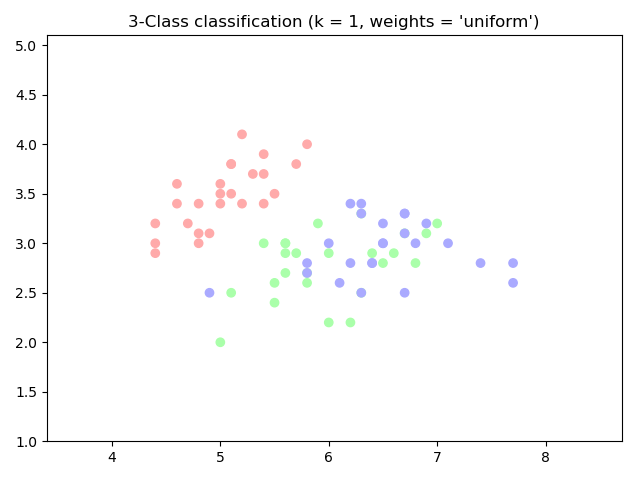
\includegraphics[scale=0.25]{KNN_iris_8_7.png}
				\caption{E8.4 accuracy = 100.00 \%}
				\label{E8.4}
			\end{minipage}
			\begin{minipage}{0.5\linewidth}
				\centering
				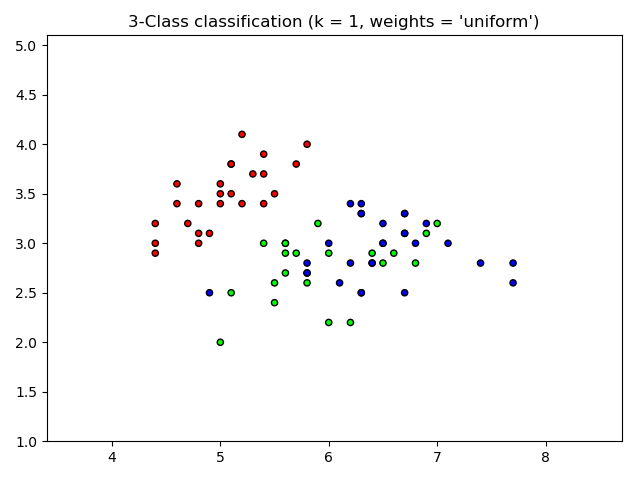
\includegraphics[scale=0.25]{KNN_iris_8_8.png}
				\caption{E8.4 accuracy = 100.00 \%}
				\label{E8.4}
			\end{minipage}
		\end{figure}
		\FloatBarrier
	\subsection{Eksperyment 9}
		\begin{figure}[H]
			\begin{minipage}{0.5\linewidth}
				\centering
				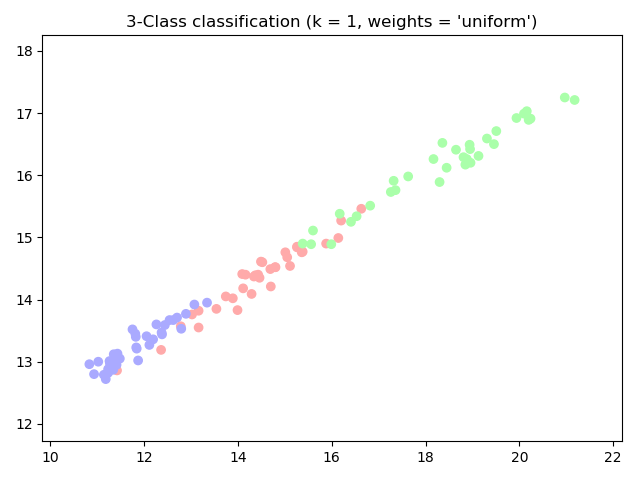
\includegraphics[scale=0.25]{KNN_seed_9_1.png}
				\caption{E9.1 accuracy = 100.00 \%}
			\end{minipage}
			\begin{minipage}{0.5\linewidth}
				\centering
				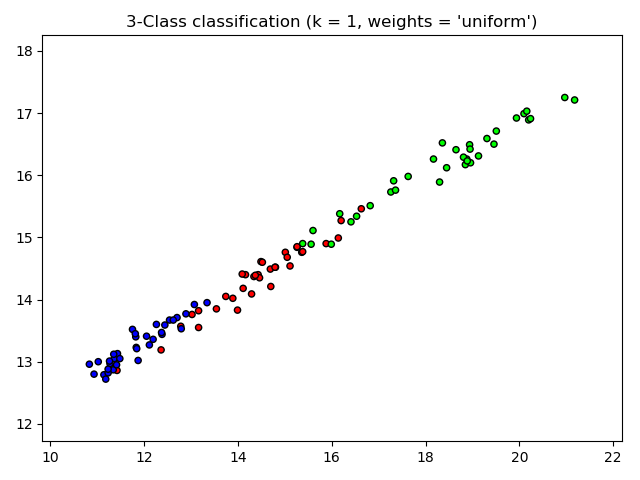
\includegraphics[scale=0.25]{KNN_seed_9_2.png}
				\caption{E9.1 accuracy = 100.00 \%}
				\label{E9.1}
			\end{minipage}
			\begin{minipage}{0.5\linewidth}
				\centering
				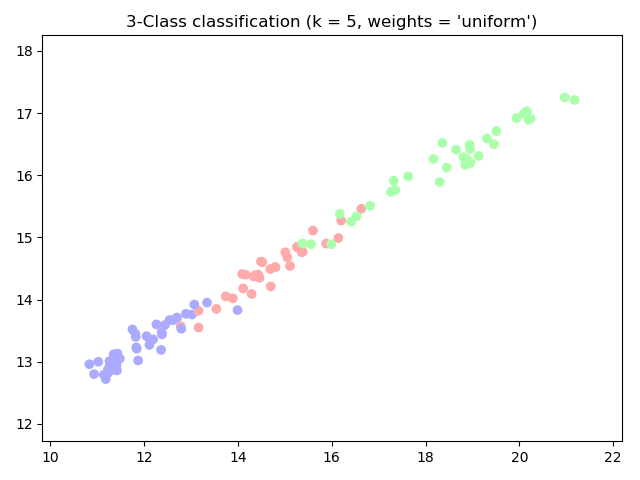
\includegraphics[scale=0.25]{KNN_seed_9_3.png}
				\caption{E9.2 accuracy = 95.24 \%}
				\label{E9.2}
			\end{minipage}
			\begin{minipage}{0.5\linewidth}
				\centering
				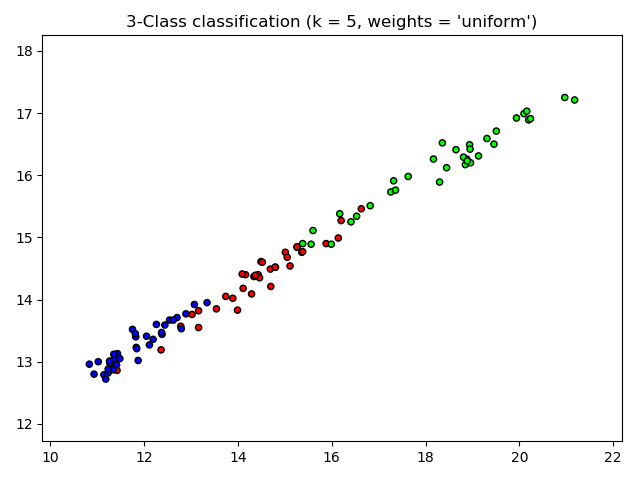
\includegraphics[scale=0.25]{KNN_seed_9_4.png}
				\caption{E9.2 accuracy = 95.24 \%}
				\label{E9.2}
			\end{minipage}
			\begin{minipage}{0.5\linewidth}
				\centering
				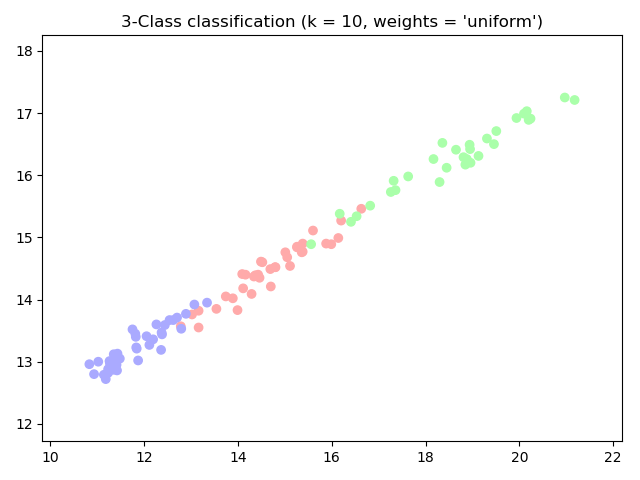
\includegraphics[scale=0.25]{KNN_seed_9_5.png}
				\caption{E9.3 accuracy = 93.33 \%}
				\label{E9.3}
			\end{minipage}
			\begin{minipage}{0.5\linewidth}
				\centering
				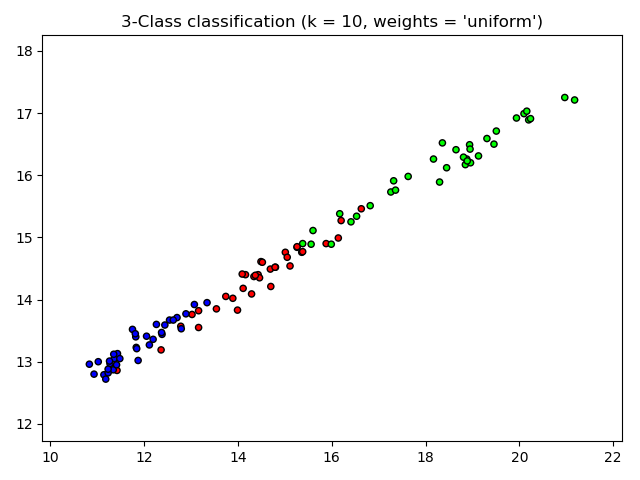
\includegraphics[scale=0.25]{KNN_seed_9_6.png}
				\caption{E9.3 accuracy = 93.33 \%}
				\label{E9.3}
			\end{minipage}
			\begin{minipage}{0.5\linewidth}
				\centering
				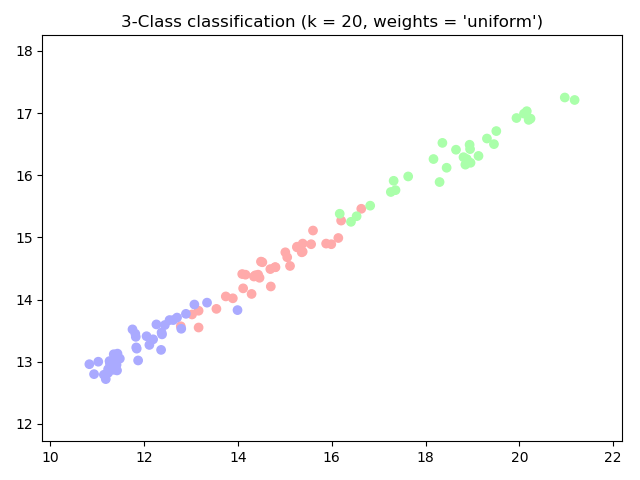
\includegraphics[scale=0.25]{KNN_seed_9_7.png}
				\caption{E9.4 accuracy = 95.24 \%}
				\label{E9.4}
			\end{minipage}
			\begin{minipage}{0.5\linewidth}
				\centering
				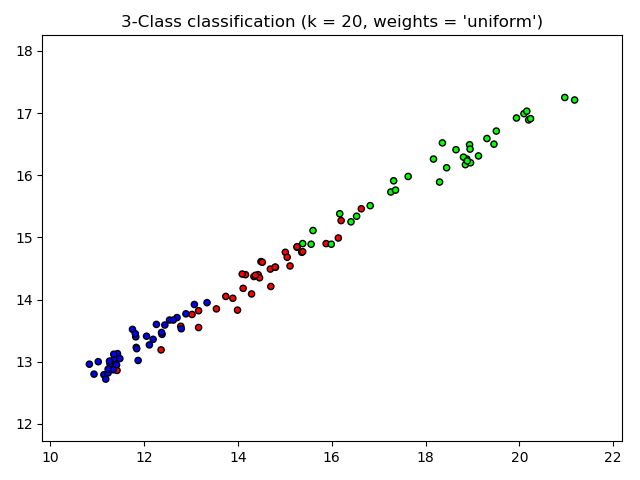
\includegraphics[scale=0.25]{KNN_seed_9_8.png}
				\caption{E9.4 accuracy = 95.24 \%}
				\label{E9.4}
			\end{minipage}
		\end{figure}
		\FloatBarrier
	\subsection{Eksperyment 10}
		\begin{figure}[H]
			\begin{minipage}{0.5\linewidth}
				\centering
				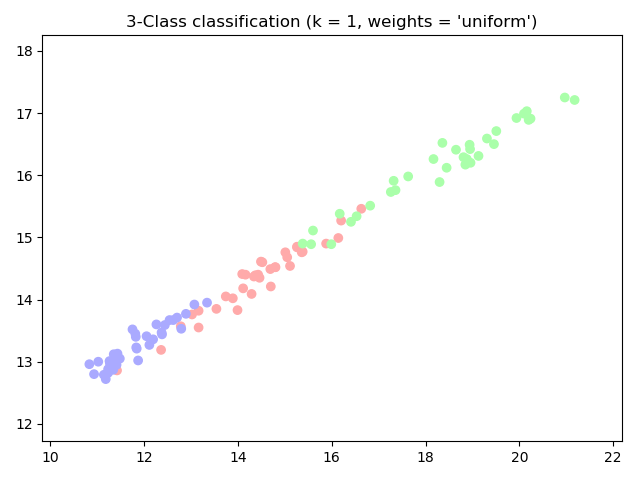
\includegraphics[scale=0.25]{KNN_seed_10_1.png}
				\caption{E10.1 accuracy = 100.00 \%, Weight - uniform}
			\end{minipage}
			\begin{minipage}{0.5\linewidth}
				\centering
				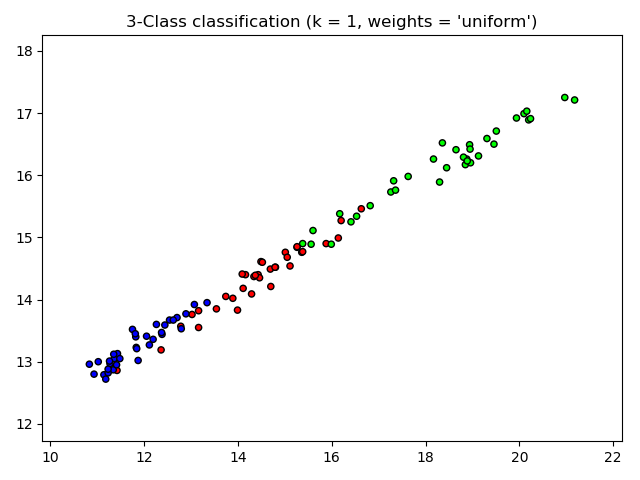
\includegraphics[scale=0.25]{KNN_seed_10_2.png}
				\caption{E10.1 accuracy = 100.00 \%, Weight - uniform}
				\label{E10.1}
			\end{minipage}
			\begin{minipage}{0.5\linewidth}
				\centering
				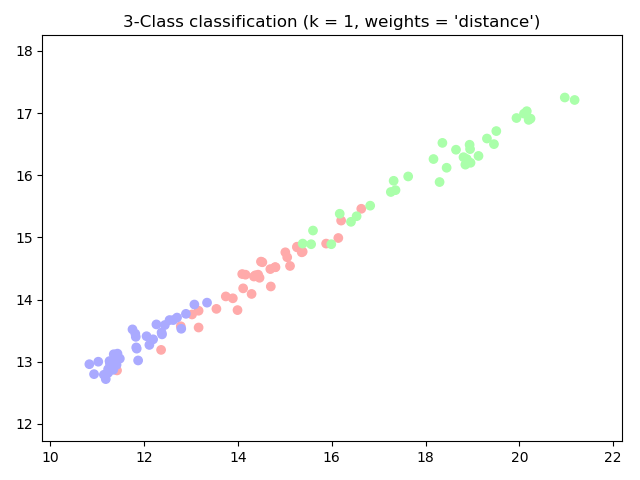
\includegraphics[scale=0.25]{KNN_seed_10_3.png}
				\caption{E10.1 accuracy = 100.00 \% Weight - distance}
				\label{E10.1}
			\end{minipage}
			\begin{minipage}{0.5\linewidth}
				\centering
				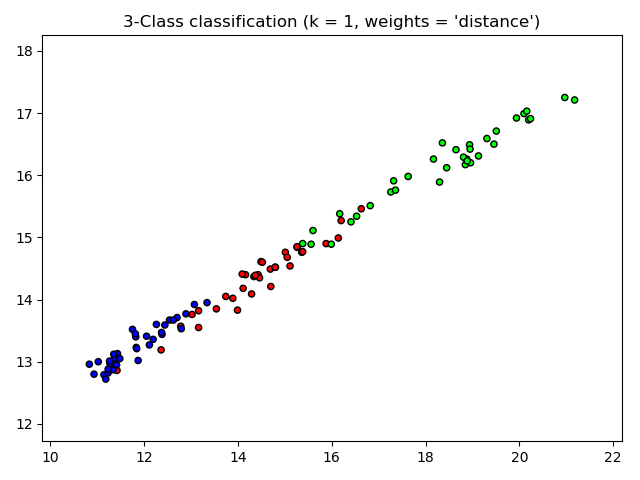
\includegraphics[scale=0.25]{KNN_seed_10_4.png}
				\caption{E10.1 accuracy = 100.00 \% Weight - distance}
				\label{E10.1}
			\end{minipage}
			\begin{minipage}{0.5\linewidth}
				\centering
				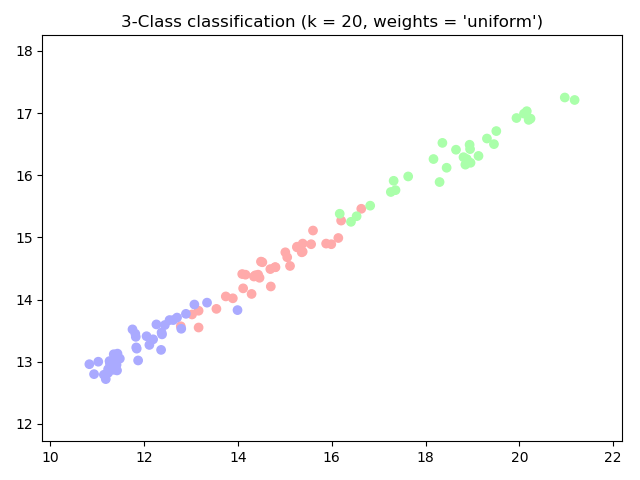
\includegraphics[scale=0.25]{KNN_seed_10_5.png}
				\caption{E10.2 accuracy = 93.33 \% Weight - uniform}
				\label{E10.2}
			\end{minipage}
			\begin{minipage}{0.5\linewidth}
				\centering
				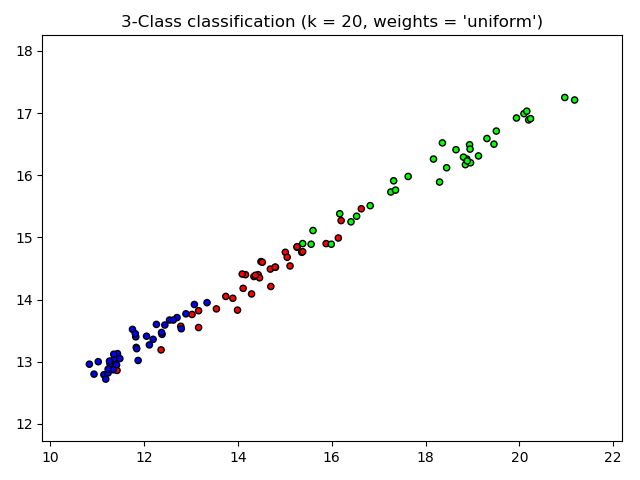
\includegraphics[scale=0.25]{KNN_seed_10_6.png}
				\caption{E10.2 accuracy = 93.33 \% Weight - uniform}
				\label{E10.2}
			\end{minipage}
			\begin{minipage}{0.5\linewidth}
				\centering
				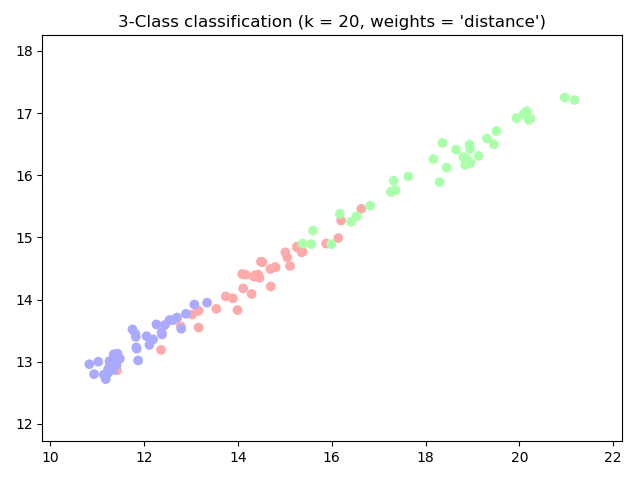
\includegraphics[scale=0.25]{KNN_seed_10_7.png}
				\caption{E10.2 accuracy = 100.00 \% Weight - distance}
				\label{E10.2}
			\end{minipage}
			\begin{minipage}{0.5\linewidth}
				\centering
				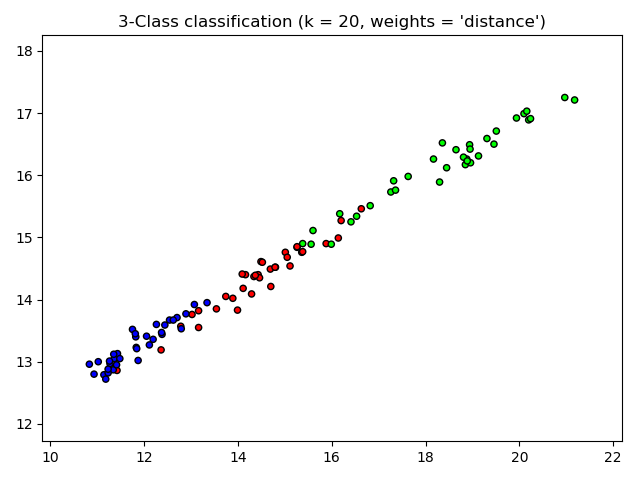
\includegraphics[scale=0.25]{KNN_seed_10_8.png}
				\caption{E10.2 accuracy = 100.00 \% Weight - distance}
				\label{E10.2}
			\end{minipage}
			\begin{minipage}{0.5\linewidth}
				\centering
				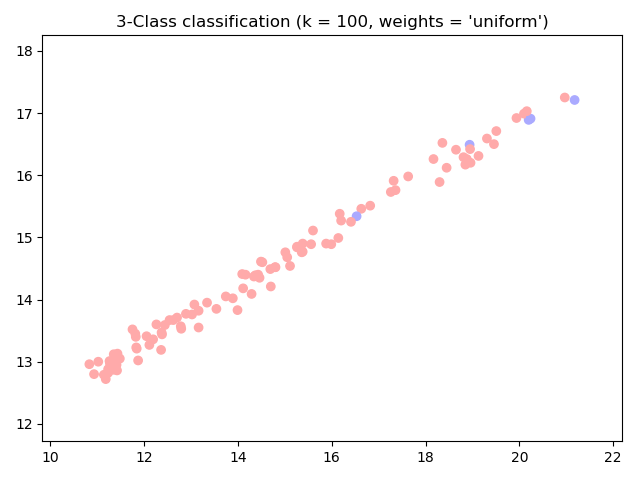
\includegraphics[scale=0.25]{KNN_seed_10_9.png}
				\caption{E10.3 accuracy = 38.10 \% Weight - uniform}
				\label{E10.3}
			\end{minipage}
			\begin{minipage}{0.5\linewidth}
				\centering
				\includegraphics[scale=0.25]{KNN_seed_10_10.png}
				\caption{E10.3 accuracy = 38.10 \% Weight - uniform}
				\label{E10.3}
			\end{minipage}
			\begin{minipage}{0.5\linewidth}
				\centering
				\includegraphics[scale=0.25]{KNN_seed_10_11.png}
				\caption{E10.3 accuracy = 100.00 \% Weight - distance}
				\label{E10.3}
			\end{minipage}
			\begin{minipage}{0.5\linewidth}
				\centering
				\includegraphics[scale=0.25]{KNN_seed_10_12.png}
				\caption{E10.3 accuracy = 100.00 \% Weight - distance}
				\label{E10.3}
			\end{minipage}
		\end{figure}
		\FloatBarrier
			

\section{Dyskusja}
W pierwszym eksperymencie pierwszym możemy zauważyć, iż dwa neurony w ukrytej warstwie daje tak samo dobry wynik jak 7 i 12 neuronów. Jednak przy 20 neuronach możemy zuważyć, że procesz uczenia jest znacznie wolniejszy. Dla tak wielu neurów błąd całkowity jest czterokrotnie większy oraz wyznaczył dwukrotnie mniej prawdziwych klas dla zbioru testowego.


W eksperymentach 2 i 5 możemy zauważyć, iż wartość learning rate ma duże znaczenie na szubkość uczenia. W otrzymanych wynikach zuważamy, że im większa wartość tym większy krok uczenia, więc szybsze początkowe uczenie.


W eksperymentach 3 i 6 obserwujemy wpływ momentum na szybkość uczenia. Wartość ta znacząco przyspiesza szybkość uczenia. Zbyt mała wartość nie daje różnicy w wyniku, jednak zbyt duża może prowadzić do wykonywania większych zmian na wagach niż pożądane.


W eksperymencie 4 rozpatrujemy wpływ liczby iteracji na końcowy wynik. Otrzymane dane sugerują iż im więcej iteracji tym lepiej. Większa liczba iteracji powinna prowadzić do lepszych wyników w niemal każdym przypadku.


Algorytm KNN - W przeprowadzonych eksperymentach 7 - 10 zauważalnym jest, że na dokładnosć przeprowadzonych badań pozytywnego wpływu nie ma zwiększona ilosć sąsiadów. Drugim ważnym aspektem jest dobrana waga. Gdy wszystkie punkty zostaną potraktowane na równi, bład oscyluje od 0 do 100 \%, jednakże gdy przyjmiemy sąsiada najbliższego badanemu punktowi jako najważniejszego bład rzadko kiedy spada ponieżej 100 \%
\section{Wnioski}
Algorytm KNN jest algorytmem optymalnym przy wprowadzeniu wagi dla sąsiadów rozpatrywanego punktu.


Algorytm sieci neuronowej posiada wiele parametrów, które należy brać pod uwagę. Moim zdaniem z łatwością możemy wyznaczyć domyślne wartości parametrów learning rate oraz momentum. Jednak dla liczby neuronów i iteracji użytkownik algorytmu musi dobierać z większą uwagą.

\begin{thebibliography}{0}
\bibitem{irisdataset}https://archive.ics.uci.edu/ml/datasets/iris
Zbiór danych dla irysów
\bibitem{seedsdataset}https://archive.ics.uci.edu/ml/datasets/seeds
Zbiór danych dla nasion
\bibitem{backPopgation}https://mattmazur.com/2015/03/17/a-step-by-step-backpropagation-example/
Back Propagation
\end{thebibliography}

\end{document}